\section{Teoria dell'Informazione}

L'informazione è un concetto molto vasto che cambia a seconda del contesto in cui lo si usa. In termini semplici: l'informazione è tutto ciò che riduce l'incertezza su un determinato evento.

Nella teoria dell'informazione, l'informazione riguarda l'imprevedibilità e non il senso di una frase. Più un messaggio è raro o inaspettato, maggiore è la quantità di informazione che trasporta.

Ipotizziamo di lanciare una moneta e di predire il risultato: "Se ti dicessi che è uscito testa, quanto saresti sorpreso?". Un bit è la risposta corretta.

Se lanciassi due monete, provassi a predire il risultato e poi ti dicessi che sono uscite due croci, quanto saresti sorpreso? \textit{A bit more}. Esattamente 1 bit in più, ovvero 2 bit.

Più un evento è probabile, meno sorpreso sei. Più la probabilità è piccola, più sarai sorpreso dal risultato se questo si verifica.

Per esprimere la quantità di sorpresa utilizziamo la lettera $I$, che sta per \textit{Information} e per ora significa "sorpresa".

L'informazione (o sorpresa) di un evento $E$ è pari a $I(E) = \log(1/P(E))$. Ma perché?

Scegliamo $1/P(E)$ perché meno un evento è probabile, più ne saremo sorpresi.

Perché usiamo il logaritmo? È una funzione che cresce al decrescere della probabilità: ad esempio, se dimezzi la probabilità, l'informazione aumenta di 1 bit. In questo modo, una probabilità di 1 su un milione è direttamente comparabile (e proporzionata in scala logaritmica) con una probabilità di 1 su 2 milioni.

L'unità di misura dell'informazione è proprio il bit.

\subsection{Esempio: Sorgente Quaternaria}

Facciamo un esempio: ipotizziamo di avere una sorgente quaternaria, il che significa che vengono emessi dei simboli. Ipotizziamo che l'emissione sia modellata tramite una variabile aleatoria $X$ il cui alfabeto è $\{0, 1, 2, 3\}$. Indichiamo con $X_{(n)}$ l'$n$-esima emissione della sorgente.

Se emettiamo una lunga stringa di simboli, possiamo contare le occorrenze e quindi valutare la frequenza di un simbolo. Per $n \to \infty$, questa frequenza di occorrenza converge alla probabilità teorica.

Sia allora $p_{X_{(n)}}(x) = p_X(x)$, con $x \in \mathcal{X}$, la \textit{probability mass function} (pmf) della generica emissione e assumiamo:

\begin{equation}
p_X(x) = 
\begin{cases} 
\frac{1}{2} & x = 0 \\ 
\frac{1}{4} & x = 1 \\ 
\frac{1}{8} & x = 2 \\ 
\frac{1}{8} & x = 3 
\end{cases}
\end{equation}

Tutti i simboli possono essere rappresentati tramite due bit: $0 \to 00, 1 \to 01, 2 \to 10, 3 \to 11$. In pratica avremo un codice a lunghezza fissa di 2 bit/simbolo. Ci chiediamo: possiamo fare di meglio?

Siamo in grado di rappresentare gli stessi simboli ma con meno bit in media? Costruiamo un codice a lunghezza variabile di questo tipo:

\begin{center}
\renewcommand{\arraystretch}{1.5}
\begin{tabular}{lcc}
\toprule
$x$ & $C_{\text{fissa}}$ & $C_{\text{variabile}}$ \\
\midrule
0 & 00 & 0 \\
1 & 01 & 10 \\
2 & 10 & 110 \\
3 & 11 & 111 \\
\bottomrule
\end{tabular}
\end{center}

L'ipotesi è: se assegniamo ai simboli più frequenti un minor numero di bit, allora in media usiamo meno bit.

Supponiamo che la nostra sorgente emetta $N$ simboli. Indichiamo con $f_N(i)$ la frequenza con cui nella stringa appare il simbolo $i$. Avremo che il numero medio di bit per simbolo è:

\begin{equation}
L_N = \sum n_{\text{bit}}(i) \cdot f_N(i)
\end{equation}

\begin{equation*}
L_N = 1 \cdot f_N(0) + 2 \cdot f_N(1) + 3 \cdot f_N(2) + 3 \cdot f_N(3) = 1.75 \text{ bit/simbolo}
\end{equation*}

Il codice a lunghezza variabile è migliore di quello a lunghezza fissa. Tuttavia, non tutti i codici vanno bene: richiediamo un'importantissima proprietà, l'\textbf{univoca decifrabilità}.

Quando usi un codice a lunghezza variabile (alcuni simboli sono codificati con 1 bit, altri magari con 3 bit), potresti avere il problema di non capire dove finisce un simbolo e dove inizia l'altro quando leggi una lunga stringa di bit (es. \texttt{01101000...}). Il codice scelto è costruito in modo tale da poter essere sempre decodificato senza ambiguità.

La domanda che ci poniamo è: perché possiamo usare meno bit per rappresentare i 4 simboli?
La risposta è che \textbf{la sorgente è molto prevedibile}: metà delle volte emette lo zero. C'è meno "sorpresa", quindi meno incertezza. Di conseguenza, \textbf{la sorgente "emette meno informazione"}.

\subsection{Misurare matematicamente l'Informazione}

Fino ad adesso abbiamo parlato di informazione ma non abbiamo ancora dato una definizione formale, proviamoci:

\textbf{Come possiamo misurare matematicamente la "quantità di informazione" $I(A)$ che riceviamo quando scopriamo che si è verificato un certo evento A?}

Shannon (il padre di questa teoria) è partito da tre ipotesi logiche, quasi ovvie:

\begin{enumerate}
    \item \textbf{Non negatività ($I(A) \ge 0$):} "L'informazione non può nuocere". Ricevere una notizia non può mai toglierti conoscenza. Nel peggiore dei casi, se ti dico una cosa che sapevi già con assoluta certezza (probabilità 100\%), l'informazione che ti do è pari a zero. Ma non sarà mai un numero negativo.
    
    \item \textbf{Eventi rari (L'informazione è legata alla sorpresa):} Più un evento è improbabile, più informazione mi dà quando si verifica. In pratica stiamo implicitamente dicendo che l'informazione $I(A)$ deve scendere se la probabilità $P(A)$ sale, e viceversa. È una funzione decrescente della probabilità.
    
    \item \textbf{Indipendenza (Additività dell'informazione):} Se ti do due notizie completamente \textit{indipendenti} (slegate tra loro), l'informazione totale che ricevi è la somma dell'informazione della prima notizia più quella della seconda: $I(A \cap B) = I(A) + I(B)$.
\end{enumerate}

\subsubsection*{Costruzione della formula}

Per ora sappiamo che l'informazione è una funzione della probabilità $I(p)$.

Sempre dall'intuizione, sappiamo che l'informazione non può essere negativa, e nel caso peggiore se l'evento è certo allora $I(p) = 0$ e $I(p) \ge 0$.

Abbiamo detto che meno un evento è probabile, più informazione ci dà. Sia $p_1 < p_2$, allora $I(p_1) > I(p_2)$. Ora dobbiamo modellare l'additività: immaginiamo due eventi \textit{completamente indipendenti} tra loro.

Se ti rivelo il risultato del primo evento, ricevi un'informazione pari a $I(p_1)$.\\
Se poi ti rivelo il risultato del secondo, ricevi un'ulteriore informazione $I(p_2)$.\\
L'informazione totale che hai ottenuto da questa "doppia notizia" deve essere per puro buon senso la somma delle due:

\begin{equation*}
I_{\text{totale}} = I(p_1) + I(p_2)
\end{equation*}

Dalla statistica di base sappiamo che se due eventi sono indipendenti, la probabilità che si verifichino \textit{entrambi contemporaneamente} è il \textbf{prodotto} delle singole probabilità: $p_{\text{totale}} = p_1 \cdot p_2$.

Ma abbiamo appena detto nella Regola 3 che l'informazione di questo evento congiunto deve essere la \textbf{somma} delle singole informazioni. Mettendo tutto insieme otteniamo il vincolo fondamentale che la formula di Shannon deve rispettare:

\begin{equation*}
I(p_1 \cdot p_2) = I(p_1) + I(p_2)
\end{equation*}

"Qual è quell'unica funzione matematica che prende due numeri, li moltiplica al suo interno, ma restituisce in uscita la somma?" Il logaritmo.

La proprietà fondamentale dei logaritmi dice che: $\log(x \cdot y) = \log(x) + \log(y)$.

Quindi, la nostra funzione misteriosa deve essere per forza un logaritmo!

\begin{equation*}
I(p) = c \cdot \log(p)
\end{equation*}

C'è un problema però: le probabilità $p$ sono sempre numeri compresi tra 0 e 1. Il logaritmo di un numero tra 0 e 1 dà sempre un risultato \textbf{negativo}. Ma noi abbiamo stabilito nella Regola 1 che l'informazione non può essere un numero negativo. Per risolvere il problema e rendere il risultato positivo, basta aggiungere un segno meno (oppure, per le proprietà dei logaritmi, mettere la probabilità al denominatore):

\begin{equation*}
I(p) = -\log(p) \quad \text{che equivale perfettamente a} \quad I(p) = \log\left(\frac{1}{p}\right)
\end{equation*}

Shannon aveva in mano l'equazione perfetta. Doveva solo scegliere quale "base" usare per il logaritmo. Poiché lavorava nei laboratori della Bell e aveva a che fare con interruttori e circuiti digitali (Acceso/Spento, 1/0), scelse di usare la \textbf{base 2}.

Decise che l'evento più elementare immaginabile — un evento con esattamente il 50\% di probabilità (come il lancio di una moneta bilanciata, $p = 1/2$) — dovesse fornire esattamente \textbf{1 unità di informazione}:

\begin{equation*}
I(0.5) = \log_2\left(\frac{1}{0.5}\right) = \log_2(2) = 1
\end{equation*}

E battezzò per la prima volta quella singola unità di misura con un nome che avrebbe cambiato il mondo: \textbf{Bit} (Binary Digit).

Pertanto, la definizione formale della quantità di informazione per un evento $A$ è:

\begin{equation}
\boxed{ i(A) \overset{\text{def}}{=} \log_2 \frac{1}{\mathbb{P}(A)} }
\end{equation}

\subsection{1. L'informazione è una Variabile Aleatoria}

Fino ad ora abbiamo calcolato l'informazione \textit{dopo} che l'evento si è verificato. Ma se io ho una sorgente che emette simboli in continuazione, prima che il simbolo venga emesso io non so quale uscirà.

Poiché l'esito è incerto (casuale), anche \textbf{la quantità di informazione $i(A)$ che riceverò è incerta}. Per questo motivo, la quantità di informazione diventa a tutti gli effetti una \textit{variabile aleatoria} (una variabile il cui valore dipende dall'esito di un fenomeno casuale).
Dato che l'informazione è una variabile aleatoria, possiamo calcolarne il valore atteso.

\subsection{Entropia: Il Valore Atteso dell'Informazione}

Assumiamo di eseguire ripetutamente un esperimento che abbia esiti possibili $\{A_1, \dots, A_N\}$. 
Siano $\{\mathbb{P}(A_i)\}_{i=1}^N$ le corrispondenti probabilità.

Ovviamente $i(A)$ è una variabile aleatoria, rappresentata dalla funzione:

\begin{equation}
i : A \in \{A_1, \dots, A_N\} \longrightarrow i(A) = \log \frac{1}{\mathbb{P}(A)} \in [0, +\infty[
\end{equation}

Il valore medio (average value) di $i(A)$ è dunque;

\begin{equation}
\mathbb{E}[i(A)] = \sum_{A \in \{A_1, \dots, A_N\}} \mathbb{P}(A) \log \frac{1}{\mathbb{P}(A)}
\end{equation}

La quantità $H(\mathcal{E}) = \mathbb{E}[i(A)]$ si definisce \textbf{entropia} dell'esperimento aleatorio i cui possibili risultati sono $\{A_1, \dots, A_N\}$.

\vspace{0.5cm}

\subsubsection*{Formalizzazione tramite Variabili Aleatorie}

L'insieme $\{A_1, \dots, A_N\}$ è un insieme di eventi discreti. Possiamo modellare lo stesso concetto in modo più rigoroso usando una variabile aleatoria. Stiamo di fatto formalizzando la \textit{sorgente} di informazione:
\begin{itemize}
    \item $X$ è il nostro generatore casuale.
    \item $\mathcal{X}$ (l'alfabeto) è l'insieme di tutti i possibili simboli che la sorgente può "stampare".
    \item $M$ è il numero totale di questi simboli.
\end{itemize}

Sia $X$ una variabile aleatoria che assuma valori in un alfabeto $\mathcal{X}$. Per il momento, si supponga che la cardinalità dell'alfabeto sia finita $|\mathcal{X}| = M$ e che i simboli siano $\mathcal{X} = \{x_1, \dots, x_M\}$.

Gli eventi di interesse ora diventano le singole occorrenze $\{X = x_i\}_{i=1}^M$.
Possiamo quindi ridefinire la variabile aleatoria "informazione" in funzione della Probability Mass Function (pmf) $p_X$:

\begin{equation}
i(X) = \log \left[ \frac{1}{p_X[X(\omega)]} \right]
\end{equation}

Si definisce \textbf{entropia} della variabile aleatoria $X$ la quantità:

\begin{equation}
\boxed{ H(X) = \mathbb{E}[i(X)] = \sum_{i=1}^{M} p_X(x_i) \log \frac{1}{p_X(x_i)} }
\end{equation}

\section{Un teorema utile: La Disuguaglianza di Jensen}

Partiamo dalla definizione di entropia:
\begin{equation}
H(X) = \mathbb{E}[i(X)] \quad \text{sapendo che} \quad i(X) = \log \frac{1}{p_X(X(\omega))} \implies \mathbb{E}[i(X)] = \mathbb{E}\left[\log \frac{1}{p_X(X(\omega))}\right]
\end{equation}

Se definiamo la funzione $g(\cdot) = \log \frac{1}{p_X(\cdot)}$, allora possiamo scrivere l'entropia come $\mathbb{E}[g(X)] = \mathbb{E}[i(X)]$.

Ci domandiamo se esista una relazione matematica generale tra $\mathbb{E}[g(X)]$ e $g(\mathbb{E}[X])$. In altre parole, è lecito invertire l'ordine dell'operatore di aspettazione e della funzione $g$? 
In generale la risposta è \textbf{NO}. Questa uguaglianza è verificata se e solo se la funzione considerata è una linea retta. Poiché il logaritmo non è una retta, l'uguaglianza stretta non vale.

\subsection{Definizione Geometrica e Interpretazione}

\begin{itemize}
    \item L'uguaglianza $\mathbb{E}[g(X)] = g(\mathbb{E}[X])$ è un caso limite e vale \textbf{solo} se $g(x)$ è una funzione lineare o affine (una retta). Matematicamente, una retta ha "curvatura nulla" ed è considerata contemporaneamente sia convessa che concava.
    \item Se la funzione è \textbf{CONVESSA} (ha la forma a "U", $\cup$), la curva sta sempre \textit{al di sopra} delle sue tangenti. In questo caso vale la disuguaglianza: $\mathbb{E}[g(X)] \ge g(\mathbb{E}[X])$.
    \item Se la funzione è \textbf{CONCAVA} (ha la forma a campana, $\cap$), la curva sta sempre \textit{al di sotto} delle sue tangenti. In questo caso il verso si inverte: $\mathbb{E}[g(X)] \le g(\mathbb{E}[X])$.
\end{itemize}

\begin{center}
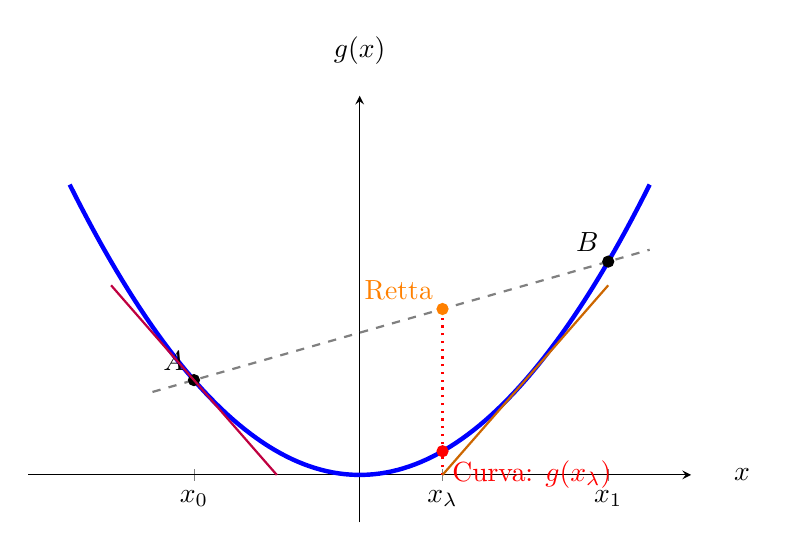
\begin{tikzpicture}
    \begin{axis}[
        width=10cm, height=7cm,
        axis lines=middle,
        xlabel={$x$}, ylabel={$g(x)$},
        xmin=-4, xmax=4, ymin=-2, ymax=16,
        xtick={-2, 1, 3},
        xticklabels={$x_0$, $x_{\lambda}$, $x_1$},
        ytick=\empty,
        every axis x label/.style={at={(ticklabel* cs:1.05)}, anchor=west,},
        every axis y label/.style={at={(ticklabel* cs:1.05)}, anchor=south,}
    ]
        % Curva convessa y = x^2
        \addplot[blue, ultra thick, domain=-3.5:3.5, samples=100] {x^2};
        
        % Retta secante tra x=-2 (y=4) e x=3 (y=9). Eq: y = x + 6
        \addplot[dashed, gray, thick, domain=-2.5:3.5] {x + 6};
        \filldraw[black] (axis cs:-2, 4) circle (2pt) node[above left] {$A$};
        \filldraw[black] (axis cs:3, 9) circle (2pt) node[above left] {$B$};
        
        % Segmento verticale nel punto intermedio lambda (es. x=1)
        % x=1 -> Curva y=1, Retta y=7
        \draw[dotted, thick, red] (axis cs:1, 0) -- (axis cs:1, 7);
        \filldraw[red] (axis cs:1, 1) circle (2pt) node[below right] {Curva: $g(x_\lambda)$};
        \filldraw[orange] (axis cs:1, 7) circle (2pt) node[above left] {Retta};

        % Tangente in x=-2: y' = 2x = -4. Eq: y - 4 = -4(x+2) -> y = -4x - 4
        \addplot[purple, thick, domain=-3:-1] {-4*x - 4};
        
        % Tangente in x=2 (y=4): y'=4. Eq: y - 4 = 4(x-2) -> y = 4x - 4
        \addplot[orange!80!black, thick, domain=1:3] {4*x - 4};

    \end{axis}
\end{tikzpicture}
\end{center}

L'interpretazione geometrica è intuitiva: prendiamo due punti qualsiasi sulla curva ($A$ e $B$) e uniamoli con un segmento rettilineo (la secante). L'espressione $\lambda x_0 + (1-\lambda)x_1$ individua un generico punto intermedio sull'asse delle ascisse, pesato da un parametro $\lambda \in [0,1]$ (che funge da "percentuale" di spostamento tra i due estremi). 

La disuguaglianza afferma che, per una funzione convessa, l'ordinata della curva in quel punto intermedio starà sempre \textit{più in basso} (o al limite coinciderà) rispetto all'ordinata del segmento secante soprastante.

Ovvero: $g(\lambda x_0 + (1-\lambda)x_1) <= \lambda g(x_0) + (1-\lambda)g(x_1)$
\subsection{Dalla Geometria al Valore Atteso}

La \textbf{Disuguaglianza di Jensen} generalizza questo concetto. Invece di calcolare una semplice media pesata tra due soli punti fisici utilizzando $\lambda$, si estende il ragionamento a \textit{tutti} i possibili valori assunti da una variabile aleatoria $X$. Questa "media globale", ponderata sulle probabilità, è per definizione il \textbf{Valore Atteso $\mathbb{E}[\cdot]$}.

Pertanto:
\begin{itemize}
    \item Se la funzione è \textbf{CONVESSA} ($\cup$): $\mathbb{E}[g(X)] \ge g(\mathbb{E}[X])$ \\
    \textit{Significato pratico:} La media dei risultati della funzione è sempre maggiore o uguale al risultato della funzione applicata alla media.
    \item Se la funzione è \textbf{CONCAVA} ($\cap$): $\mathbb{E}[g(X)] \le g(\mathbb{E}[X])$ \\
    \textit{Significato pratico:} La media dei risultati della funzione è sempre minore o uguale al risultato della funzione applicata alla media.
\end{itemize}

\subsection{Il Limite Massimo dell'Entropia}

Applichiamo ora il teorema per determinare un limite superiore all'Entropia. Abbiamo visto che:
\begin{equation}
H(X) = \mathbb{E}\left[\log \frac{1}{p_X[X(\omega)]}\right]
\end{equation}

Introduciamo un cambio di variabile e definiamo una nuova variabile aleatoria $Y$ pari all'inverso della probabilità: $Y(\omega) = \frac{1}{p_X[X(\omega)]}$. 
In questo modo, la formula dell'entropia diventa una scrittura molto più pulita: $H(X) = \mathbb{E}[\log Y]$.

Calcoliamo innanzitutto il valore atteso di questa nuova variabile $Y$:
\begin{equation}
\mathbb{E}[Y] = \sum_{x \in \mathcal{X}} \left( \frac{1}{p_X(x)} \right) p_X(x) = \sum_{x \in \mathcal{X}} 1 = |\mathcal{X}| = M
\end{equation}
La media di $Y$ è esattamente pari a $M$, ovvero il numero totale di simboli (eventi) possibili nel nostro alfabeto.

Sappiamo dall'analisi matematica che la derivata seconda del logaritmo è strettamente negativa ($\frac{d^2 \log y}{dy^2} = -\frac{1}{y^2} < 0$), per cui la funzione $\log(y)$ è globalmente \textbf{concava} $\forall y > 0$.
Questo ci autorizza formalmente ad applicare la Disuguaglianza di Jensen usando il segno \textit{minore o uguale}:
\begin{equation}
\mathbb{E}[\log Y] \le \log(\mathbb{E}[Y])
\end{equation}

Sostituendo i valori che abbiamo ricavato:
\begin{itemize}
    \item A sinistra dell'equazione, $\mathbb{E}[\log Y]$ è per definizione la nostra Entropia $H(X)$.
    \item A destra dell'equazione, sapendo che $\mathbb{E}[Y] = |\mathcal{X}|$, otteniamo $\log|\mathcal{X}|$.
\end{itemize}

Otteniamo così il teorema fondamentale:
\begin{equation}
\boxed{ H(X) \le \log |\mathcal{X}| }
\end{equation}

Questo risultato dimostra che l'entropia possiede un \textbf{tetto massimo invalicabile}: non può in alcun caso superare il logaritmo della cardinalità dell'alfabeto (il numero di eventi possibili).

\subsubsection*{Quando si ottiene la massima Entropia?}

Sapendo qual è il tetto massimo, ci chiediamo: \textit{quando l'entropia tocca esattamente quel tetto?} (Ovvero, quando l'espressione diventa un'uguaglianza rigorosa $H(X) = \log|\mathcal{X}|$?)

Come discusso in precedenza, l'uguaglianza nella Disuguaglianza di Jensen è garantita solo se l'argomento del valore atteso non è affatto una variabile aleatoria, bensì una \textbf{costante} fissa (senza incertezza).
Affinché $Y = 1/p_X(x)$ sia una costante per ogni estrazione, la probabilità $p_X(x)$ deve essere un numero fisso e identico per tutti i possibili eventi. 

Se ho $|\mathcal{X}|$ eventi e tutti devono avere la stessa identica probabilità, affinché la somma faccia 1, quella probabilità deve necessariamente essere $\frac{1}{|\mathcal{X}|}$ (esattamente come la probabilità $\frac{1}{6}$ per ogni singola faccia di un dado onesto).

\begin{quote}
\textbf{Conclusione:} Tra tutte le infinite distribuzioni di probabilità possibili, la \textbf{distribuzione uniforme} è l'unica che fornisce il valore più alto possibile di entropia. Essa rappresenta lo stato di \textbf{massima incertezza} concepibile per quel dato sistema.
\end{quote}

\section{Divergenza di Kullback-Leibler (Entropia Relativa)}

Oltre a misurare l'incertezza intrinseca di una singola sorgente dati tramite l'Entropia, nella Teoria dell'Informazione è fondamentale poter confrontare \textit{due diverse distribuzioni di probabilità}. 

A questo scopo si introduce la \textbf{Divergenza di Kullback-Leibler (KL)}, chiamata anche \textbf{Entropia Relativa}. In parole semplici, questo strumento matematico serve a rispondere a una domanda pratica cruciale:
\begin{quote}
\textit{"Se io credo (o stimo) che un fenomeno segua la distribuzione di probabilità $p_2$, ma nella realtà il fenomeno segue la distribuzione vera $p_1$, quanta informazione perdo (o quanta 'sorpresa' in più ottengo) a causa del mio errore di stima?"}
\end{quote}

\subsection{Definizione Formale}

Si consideri un alfabeto discreto $\mathcal{X}$. Siano $p_1(x)$ e $p_2(x)$ due funzioni di massa di probabilità (PMF) definite su questo stesso alfabeto.

Si definisce \textit{entropia relativa} (o divergenza, o distanza di Kullback-Leibler) tra la distribuzione vera $p_1(\cdot)$ e la distribuzione stimata $p_2(\cdot)$ la seguente quantità:

\begin{equation}
\label{eq:kl_divergence}
D(p_1 \parallel p_2) = \sum_{x \in \mathcal{X}} p_1(x) \log \left[ \frac{p_1(x)}{p_2(x)} \right] = \mathbb{E}_{p_1} \left[ \log \frac{p_1(X)}{p_2(X)} \right]
\end{equation}

Osservando la formula, il comportamento base è intuitivo: se per un dato evento $x$ le due probabilità fossero identiche ($p_1(x) = p_2(x)$), la frazione varrebbe esattamente $1$. Poiché il logaritmo di $1$ è zero ($\log(1) = 0$), quel termine non contribuirebbe alla sommatoria. 
Di conseguenza, se le distribuzioni sono perfettamente uguali in ogni punto, la divergenza totale è zero. Se invece differiscono, il rapporto crea un valore che fa crescere la sommatoria.

\subsection{Il problema dell'Asimmetria: Non è una vera "Distanza"}

Spesso, in modo improprio, si sente parlare della KL come di una "distanza" tra distribuzioni. Tuttavia, nella geometria classica, affinché una misura possa essere definita formalmente come \textit{distanza} (o metrica), deve obbligatoriamente rispettare la proprietà di simmetria. 

Nella vita reale, se misuro la distanza da Roma a Milano, ottengo esattamente lo stesso valore della distanza da Milano a Roma. 
Invece, \textbf{la Divergenza KL NON è simmetrica}:
\begin{equation}
D(p_1 \parallel p_2) \neq D(p_2 \parallel p_1)
\end{equation}

Il motivo logico è legato al concetto di informazione spiegato all'inizio: l'errore (o inefficienza) che commetto se la realtà è $p_1$ e io stimo $p_2$, non è uguale all'errore che commetto se la realtà fosse $p_2$ e io stimassi $p_1$. Il "peso" dell'errore dipende da quale sia la distribuzione vera che governa gli eventi (che nella formula \ref{eq:kl_divergence} agisce come termine moltiplicativo esterno al logaritmo).

\subsection{Proprietà Fondamentali della Divergenza KL}

Per comodità di notazione, indichiamo d'ora in poi due generiche distribuzioni con $p$ e $q$. La Divergenza di Kullback-Leibler gode delle seguenti proprietà matematiche:

\begin{itemize}
    \item \textbf{Non-negatività (sempre positiva o zero):} La "distanza" informativa tra due teorie non può mai essere un valore negativo. L'errore peggiore possibile tende a infinito, l'errore minimo (la perfezione) è zero.
    \begin{equation*}
        D(p \parallel q) \ge 0
    \end{equation*}
    
    \item \textbf{Identità (Zero assoluto):} La divergenza vale zero \textbf{se e solo se} le due distribuzioni sono perfette copie l'una dell'altra per ogni simbolo dell'alfabeto.
    \begin{equation*}
        D(p \parallel q) = 0 \iff p(x) = q(x) \quad \forall x \in \mathcal{X}
    \end{equation*}
    
    \item \textbf{Asimmetria (non è una vera metrica):} Come discusso in precedenza, scambiare l'ordine degli argomenti cambia il risultato. Calcolare l'inefficienza partendo da $p$ per arrivare a $q$ non dà lo stesso risultato del percorso inverso.
    \begin{equation*}
        D(p \parallel q) \neq D(q \parallel p)
    \end{equation*}
    
    \item \textbf{Convessità (mischiare riduce le differenze):} Se si prendono due coppie di distribuzioni ($(p_1, q_1)$ e $(p_2, q_2)$) e le si mescola attraverso una media pesata (con parametro $\lambda \in [0,1]$), la divergenza totale del "miscuglio" sarà sempre minore o uguale alla media delle loro divergenze iniziali. In termini pratici, mescolare i dati "appiattisce" le specificità e riduce le distanze relative.
    \begin{equation*}
        D(\lambda p_1 + (1-\lambda)p_2 \parallel \lambda q_1 + (1-\lambda)q_2) \le \lambda D(p_1 \parallel q_1) + (1-\lambda)D(p_2 \parallel q_2)
    \end{equation*}
\end{itemize}